\documentclass[a4paper,10pt]{scrartcl}
\usepackage[utf8]{inputenc}
\usepackage{amsmath}
\usepackage{fancyhdr}
\pagestyle{fancy}
\usepackage{dsfont}
\usepackage{amsfonts}
\usepackage{amsthm}
\usepackage{graphicx}
\usepackage[small,nooneline,bf,hang]{caption2}
\usepackage{float}
\usepackage{hyperref}

%opening
\title{Non Negative Matrix Factorization C-Library 0.96}



\begin{document}

\fancyhead{}
\rhead{performance comparison}
\lhead{NNMF C-Library 0.96}


\maketitle

	\paragraph{Hardware specifications}


	The following runtime comparisons were run on a SUN FIRE X4600 M2 with following hardware specifications:
	\newline

	\begin{itemize}
	\item	8 AMD Opteron 8356 Quad-Core processors with 3.2 GHz and 2MB L3 cache
	\item	CPUs are connected to each other by a HyperTransport link running at 8 GB/second
	\item	32GB of main memory (DDR-II 666)
	\end{itemize}


	\paragraph{Notes on performance measurements}

	The timings were generated using the C function \texttt{gettimeofday}. Actually measured was the pure computational time, ignoring loading/storing from/to disk which is comparable to the built-in MATLAB function \texttt{nnmf}.


	CPU core usage was gathered using the GNU \texttt{top} utility. For every run the number of utilized cores is listed. Referring to this linkage of ATLAS 3.8.3 showed a salient behavior; the number of used cores was very varying with previously used cores becoming unused and different cores starting to get used frequently. Therefore for this linkage the maximum number of cores simultaneously used during the execution is stated.
	
	
	
	\begin{figure}
		\label{Figure1}	
		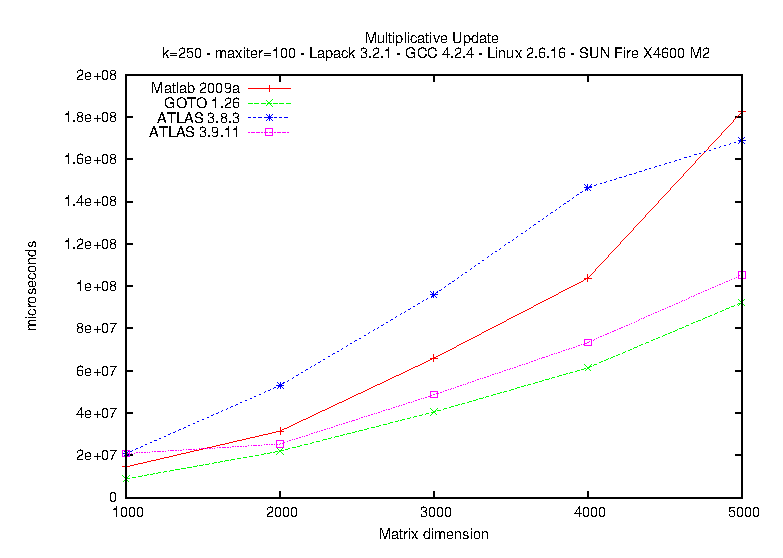
\includegraphics{nmf_mu.eps}\newline

		
		\textbf{Number of cores used during calculation}\newline
		Note: High core usage fluctuation using ATLAS 3.8.3\newline

		\begin{tabular}{|c|c|c|c|c|c|}
			\hline
			Matrix dimension & iterations & Matlab 2009a & Goto 1.26 & ATLAS 3.8.3 & ATLAS 3.9.11\\
			\hline
			1000 & $100$ & $32$ & $32$ & $<15$ & $32$\\
			2000 & $100$ & $32$ & $32$ & $<25$ & $32$ \\
			3000 & $100$ & $32$ & $32$ & $<29$ & $32$\\
			4000 & $100$ & $32$ & $32$ & $<=32$ & $32$\\
			5000 & $100$ & $32$ & $32$ & $<=32$ & $32$\\
			\hline
		\end{tabular}
		\caption{Performance comparison for Multiplicative Update}
	\end{figure}

	



	\begin{figure}
		\label{Figure2}	
		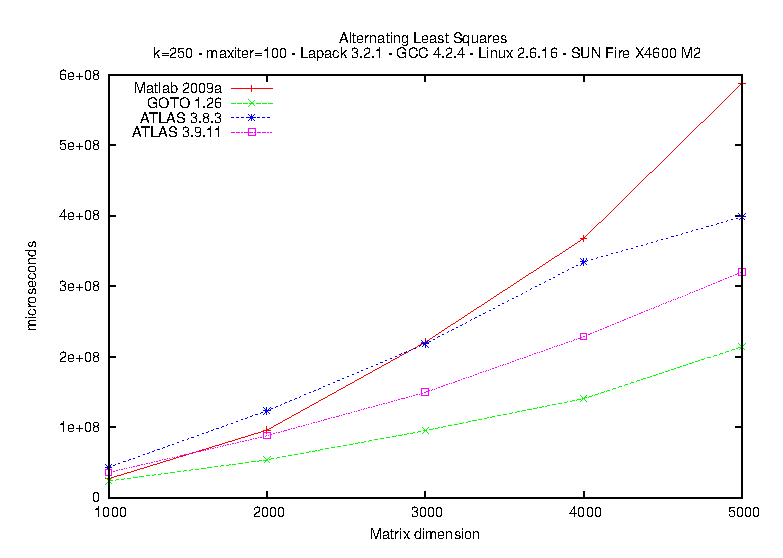
\includegraphics{nmf_als.eps}\newline

		
		\textbf{Number of cores used during calculation}\newline
		Note: High core usage fluctuation using ATLAS 3.8.3\newline

		\begin{tabular}{|c|c|c|c|c|c|}
			\hline
			Matrix dimension & iterations & Matlab 2009a & Goto 1.26 & ATLAS 3.8.3 & ATLAS 3.9.11\\
			\hline
			1000 & $100$ & $32$ & $32$ & $<12$ & $32$\\
			2000 & $100$ & $32$ & $32$ & $<20$ & $32$ \\
			3000 & $100$ & $32$ & $32$ & $<26$ & $32$\\
			4000 & $100$ & $32$ & $32$ & $<29$ & $32$\\
			5000 & $100$ & $32$ & $32$ & $<=32$ & $32$\\
			\hline
		\end{tabular}
		\caption{Performance comparison for Alternating Least Squares}
	\end{figure}

	\begin{figure}
		\label{Figure3}	
		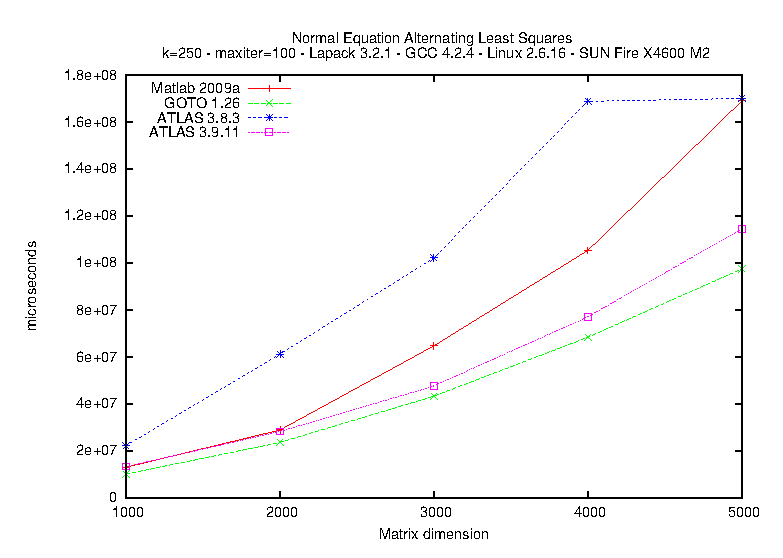
\includegraphics{nmf_neals.eps}\newline

		
		\textbf{Number of cores used during calculation}\newline
		Note: High core usage fluctuation using ATLAS 3.8.3\newline

		\begin{tabular}{|c|c|c|c|c|c|}
			\hline
			Matrix dimension & iterations & Matlab 2009a & Goto 1.26 & ATLAS 3.8.3 & ATLAS 3.9.11\\
			\hline
			1000 & $100$ & $32$ & $32$ & $<15$ & $32$\\
			2000 & $100$ & $32$ & $32$ & $<20$ & $32$ \\
			3000 & $100$ & $32$ & $32$ & $<29$ & $32$\\
			4000 & $100$ & $32$ & $32$ & $<31$ & $32$\\
			5000 & $100$ & $32$ & $32$ & $<=32$ & $32$\\
			\hline
		\end{tabular}
		\caption{Performance comparison for Normal Equation Alternating Least Squares}
	\end{figure}

	\begin{figure}
		\label{Figure4}	
		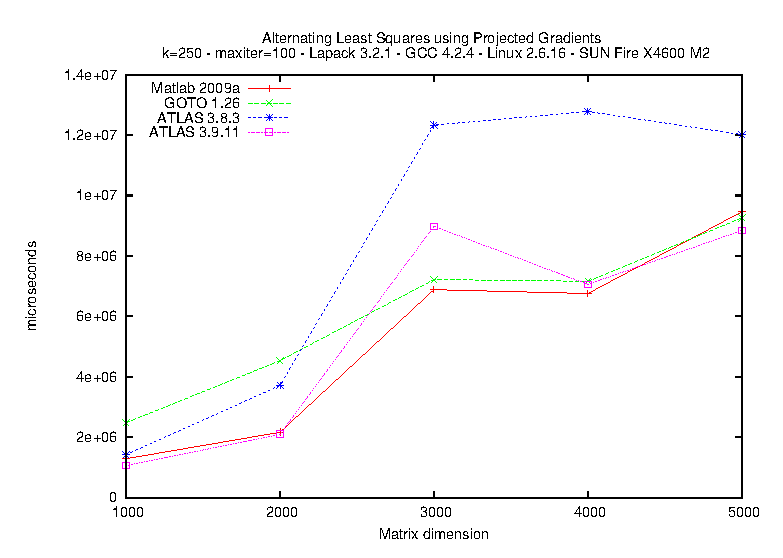
\includegraphics{nmf_alspg.eps}\newline

		
		\textbf{Number of cores used during calculation}\newline
		Note: High core usage fluctuation using ATLAS 3.8.3\newline

		\begin{tabular}{|c|c|c|c|c|c|}
			\hline
			Matrix dimension & iterations & Matlab 2009a & Goto 1.26 & ATLAS 3.8.3 & ATLAS 3.9.11\\
			\hline
			1000 & $4$ & $32$ & $32$ & $<10$ & $32$\\
			2000 & $4$ & $32$ & $32$ & $<12$ & $32$ \\
			3000 & $4$ & $32$ & $32$ & $<14$ & $32$\\
			4000 & $4$ & $32$ & $32$ & $<29$ & $32$\\
			5000 & $4$ & $32$ & $32$ & $<=32$ & $32$\\
			\hline
		\end{tabular}
		\caption{Performance comparison for Alternating Least Squares using a Projected Gradient approach}
	\end{figure}


	\begin{figure}
		\label{Figure5}	
		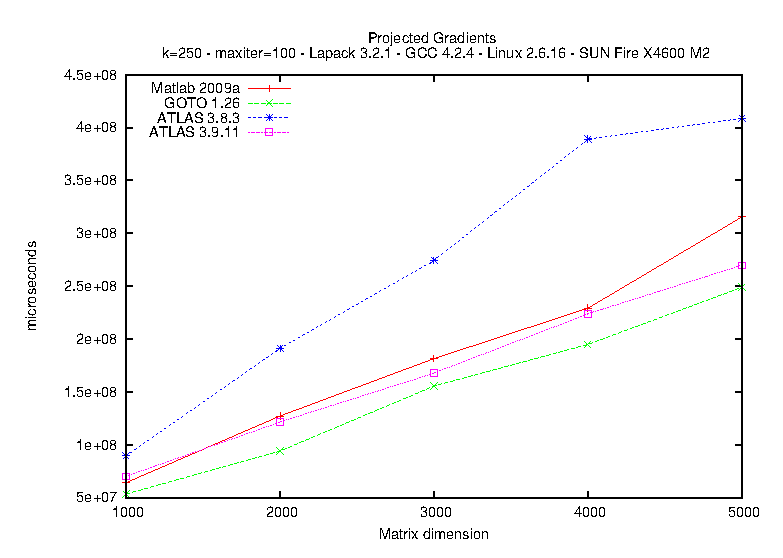
\includegraphics{nmf_pg.eps}\newline

		
		\textbf{Number of cores used during calculation}\newline
		Note: High core usage fluctuation using ATLAS 3.8.3\newline

		\begin{tabular}{|c|c|c|c|c|c|}
			\hline
			Matrix dimension & iterations & Matlab 2009a & Goto 1.26 & ATLAS 3.8.3 & ATLAS 3.9.11\\
			\hline
			1000 & $2$ & $32$ & $32$ & $8$ & $32$\\
			2000 & $2$ & $32$ & $32$ & $<11$ & $32$ \\
			3000 & $2$ & $32$ & $32$ & $<15$ & $32$\\
			4000 & $2$ & $32$ & $32$ & $<12$ & $32$\\
			5000 & $2$ & $32$ & $32$ & $<12$ & $32$\\
			\hline
		\end{tabular}
		\caption{Performance comparison for Projected Gradient}
	\end{figure}
	


\end{document}
